\section{Results} \label{sec:results}

Figure~\ref{fig:corr_pi_p} shows the same-event yield (left panel), mixed event yield (middle panel) and correlation functions (right panels) as 2D functions of $\Delta\phi$ and $\Delta y$ (top) and 1D functions of $\Delta\phi$  for the $1.5<\Delta y<2.5$ region (bottom) for all $\pi p$ events.  The same types of plots are shown for $\pi^+p$, $\pi^-p$, and $\pi\pi$ events in Figs.~\ref{fig:corr_pi+_p} through \ref{fig:corr_pi_pi}

\begin{figure}
    \centering
    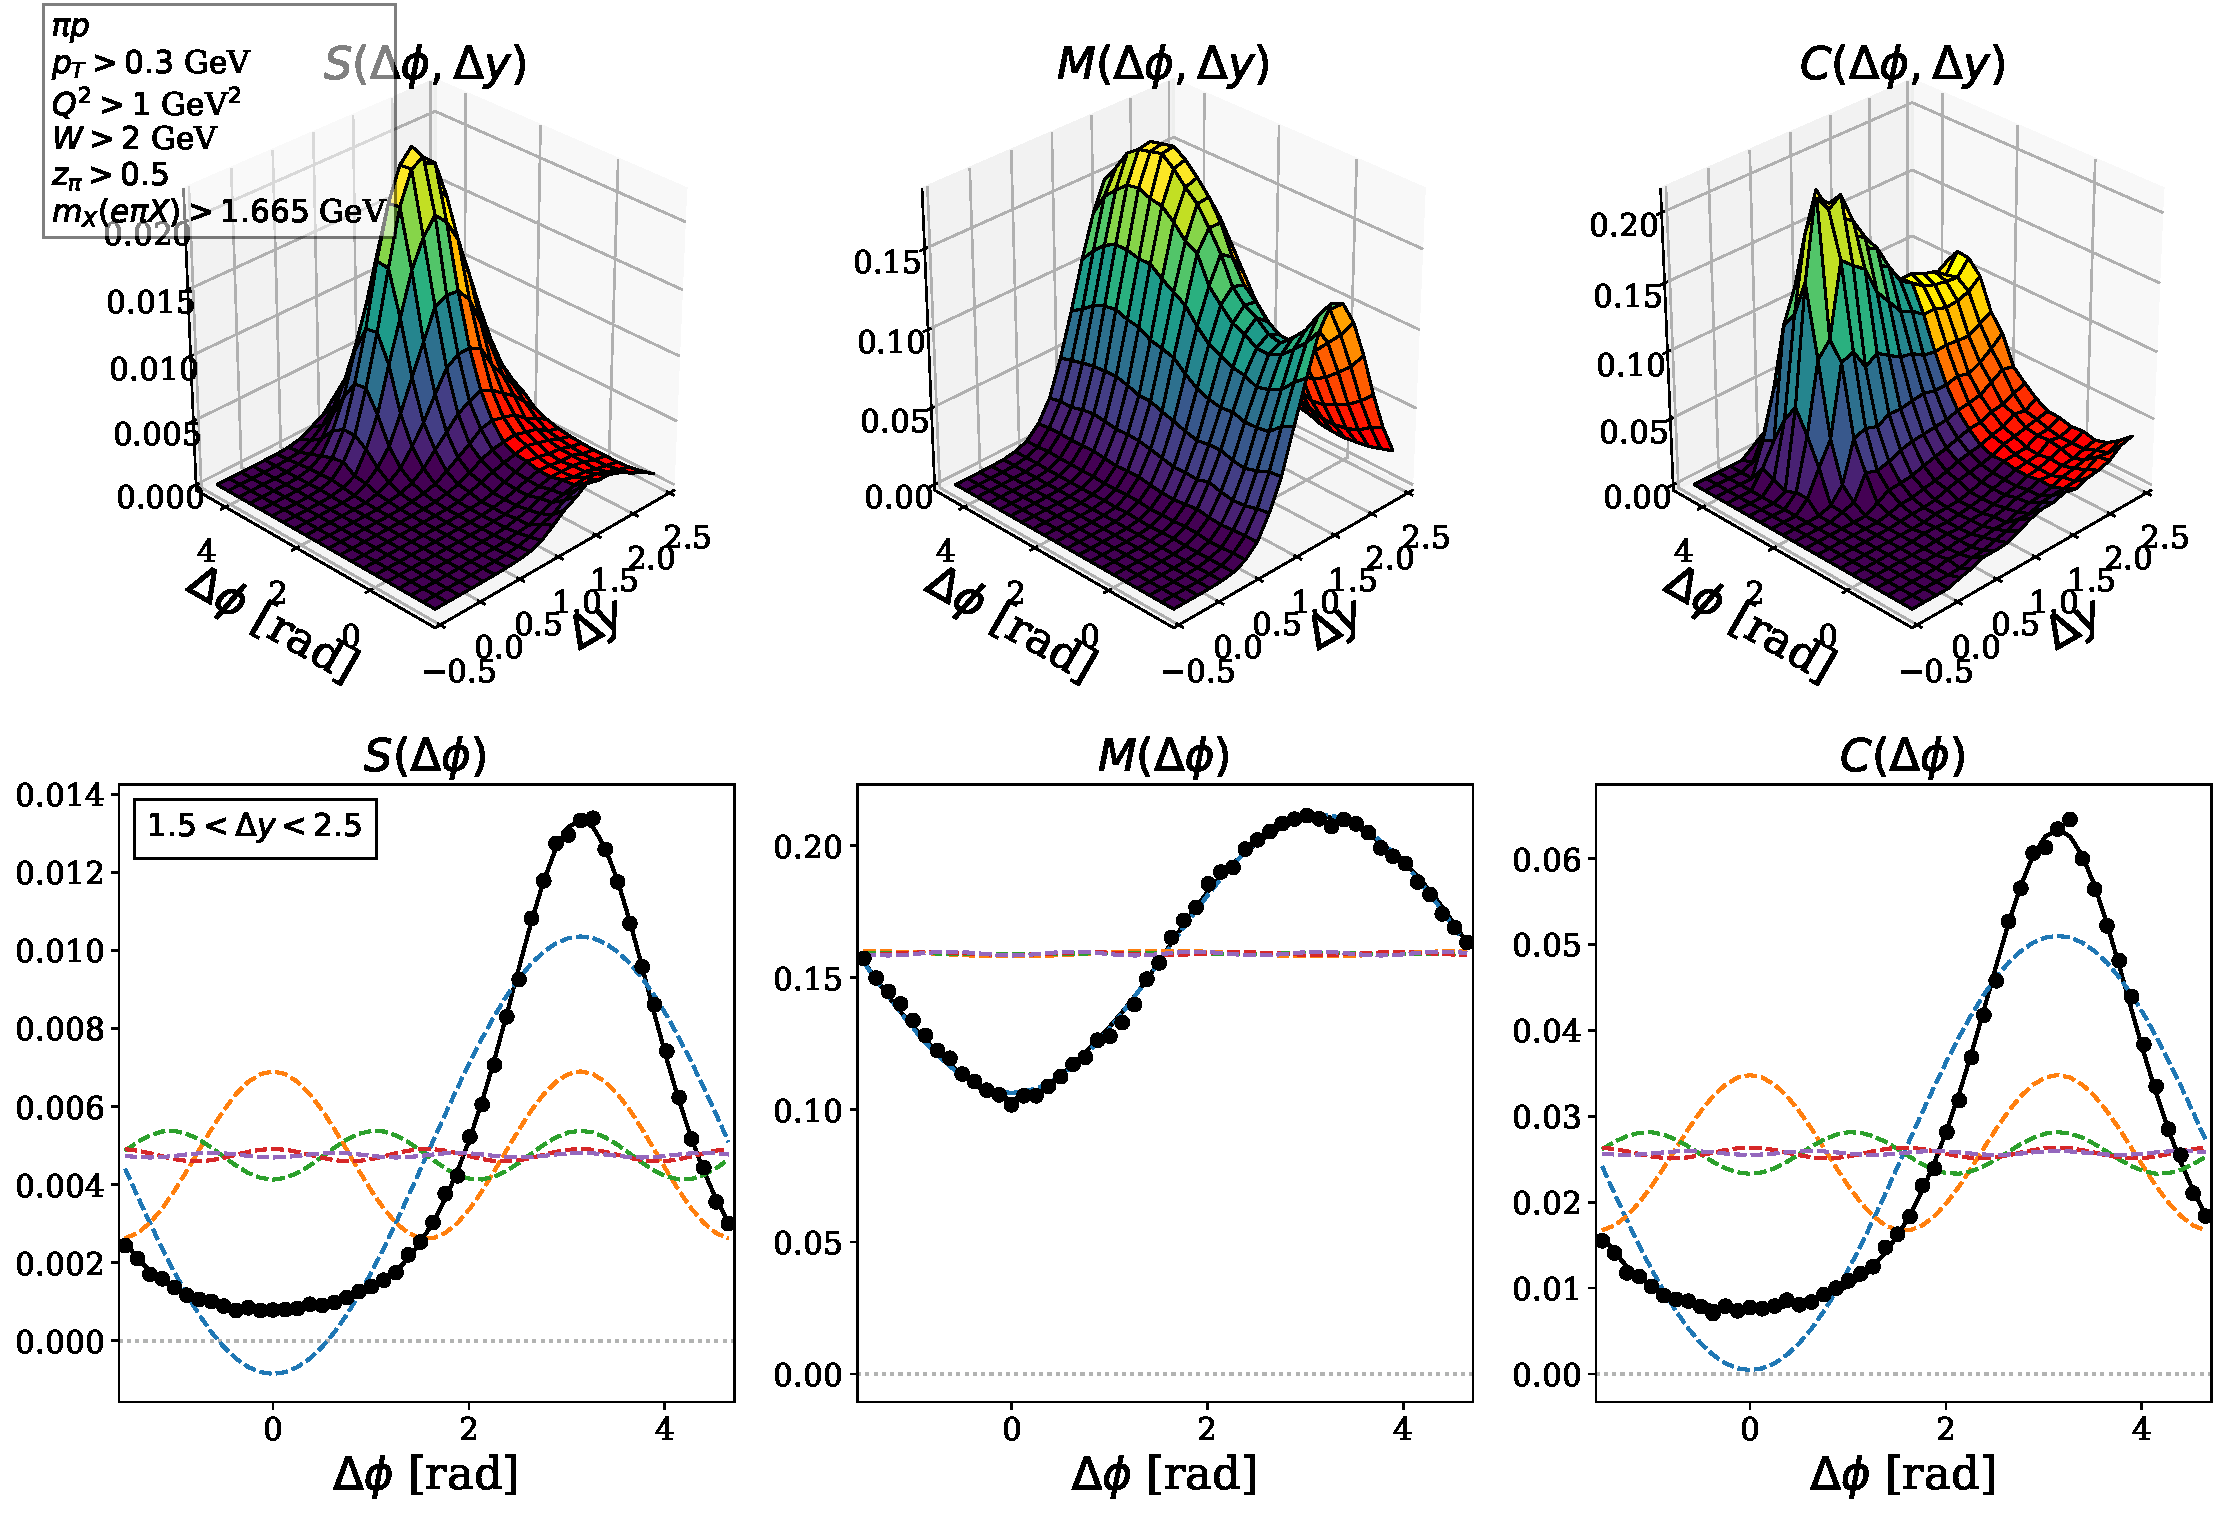
\includegraphics[width=\textwidth]{smc_pi_p.pdf}
    \caption{same-event yield (left panel), mixed event yield (middle panel) and correlation functions (right panels) as 2D functions of $\Delta\phi$ and $\Delta y$ (top) and 1D functions of $\Delta\phi$  for the $1.5<\Delta y<2.5$ region (bottom) for all $\pi p$ events.  The $1.5<\Delta y<2.5$ region is highlighted in the top row of plots using a brighter color scheme than the rest of the plot.}
    \label{fig:corr_pi_p}
\end{figure}

% \begin{figure}
%     \centering
%     \includegraphics[width=\textwidth]{dphi_vs_deta_pi+_p.pdf}
%     \caption{Same as Fig.~\ref{fig:corr_pi_p} for $\pi^+ p$ events.}
%     \label{fig:corr_pi+_p}
% \end{figure}

% \begin{figure}
%     \centering
%     \includegraphics[width=\textwidth]{dphi_vs_deta_pi-_p.pdf}
%     \caption{Same as Fig.~\ref{fig:corr_pi_p} for $\pi^- p$ events.}
%     \label{fig:corr_pi-_p}
% \end{figure}

\begin{figure}
    \centering
    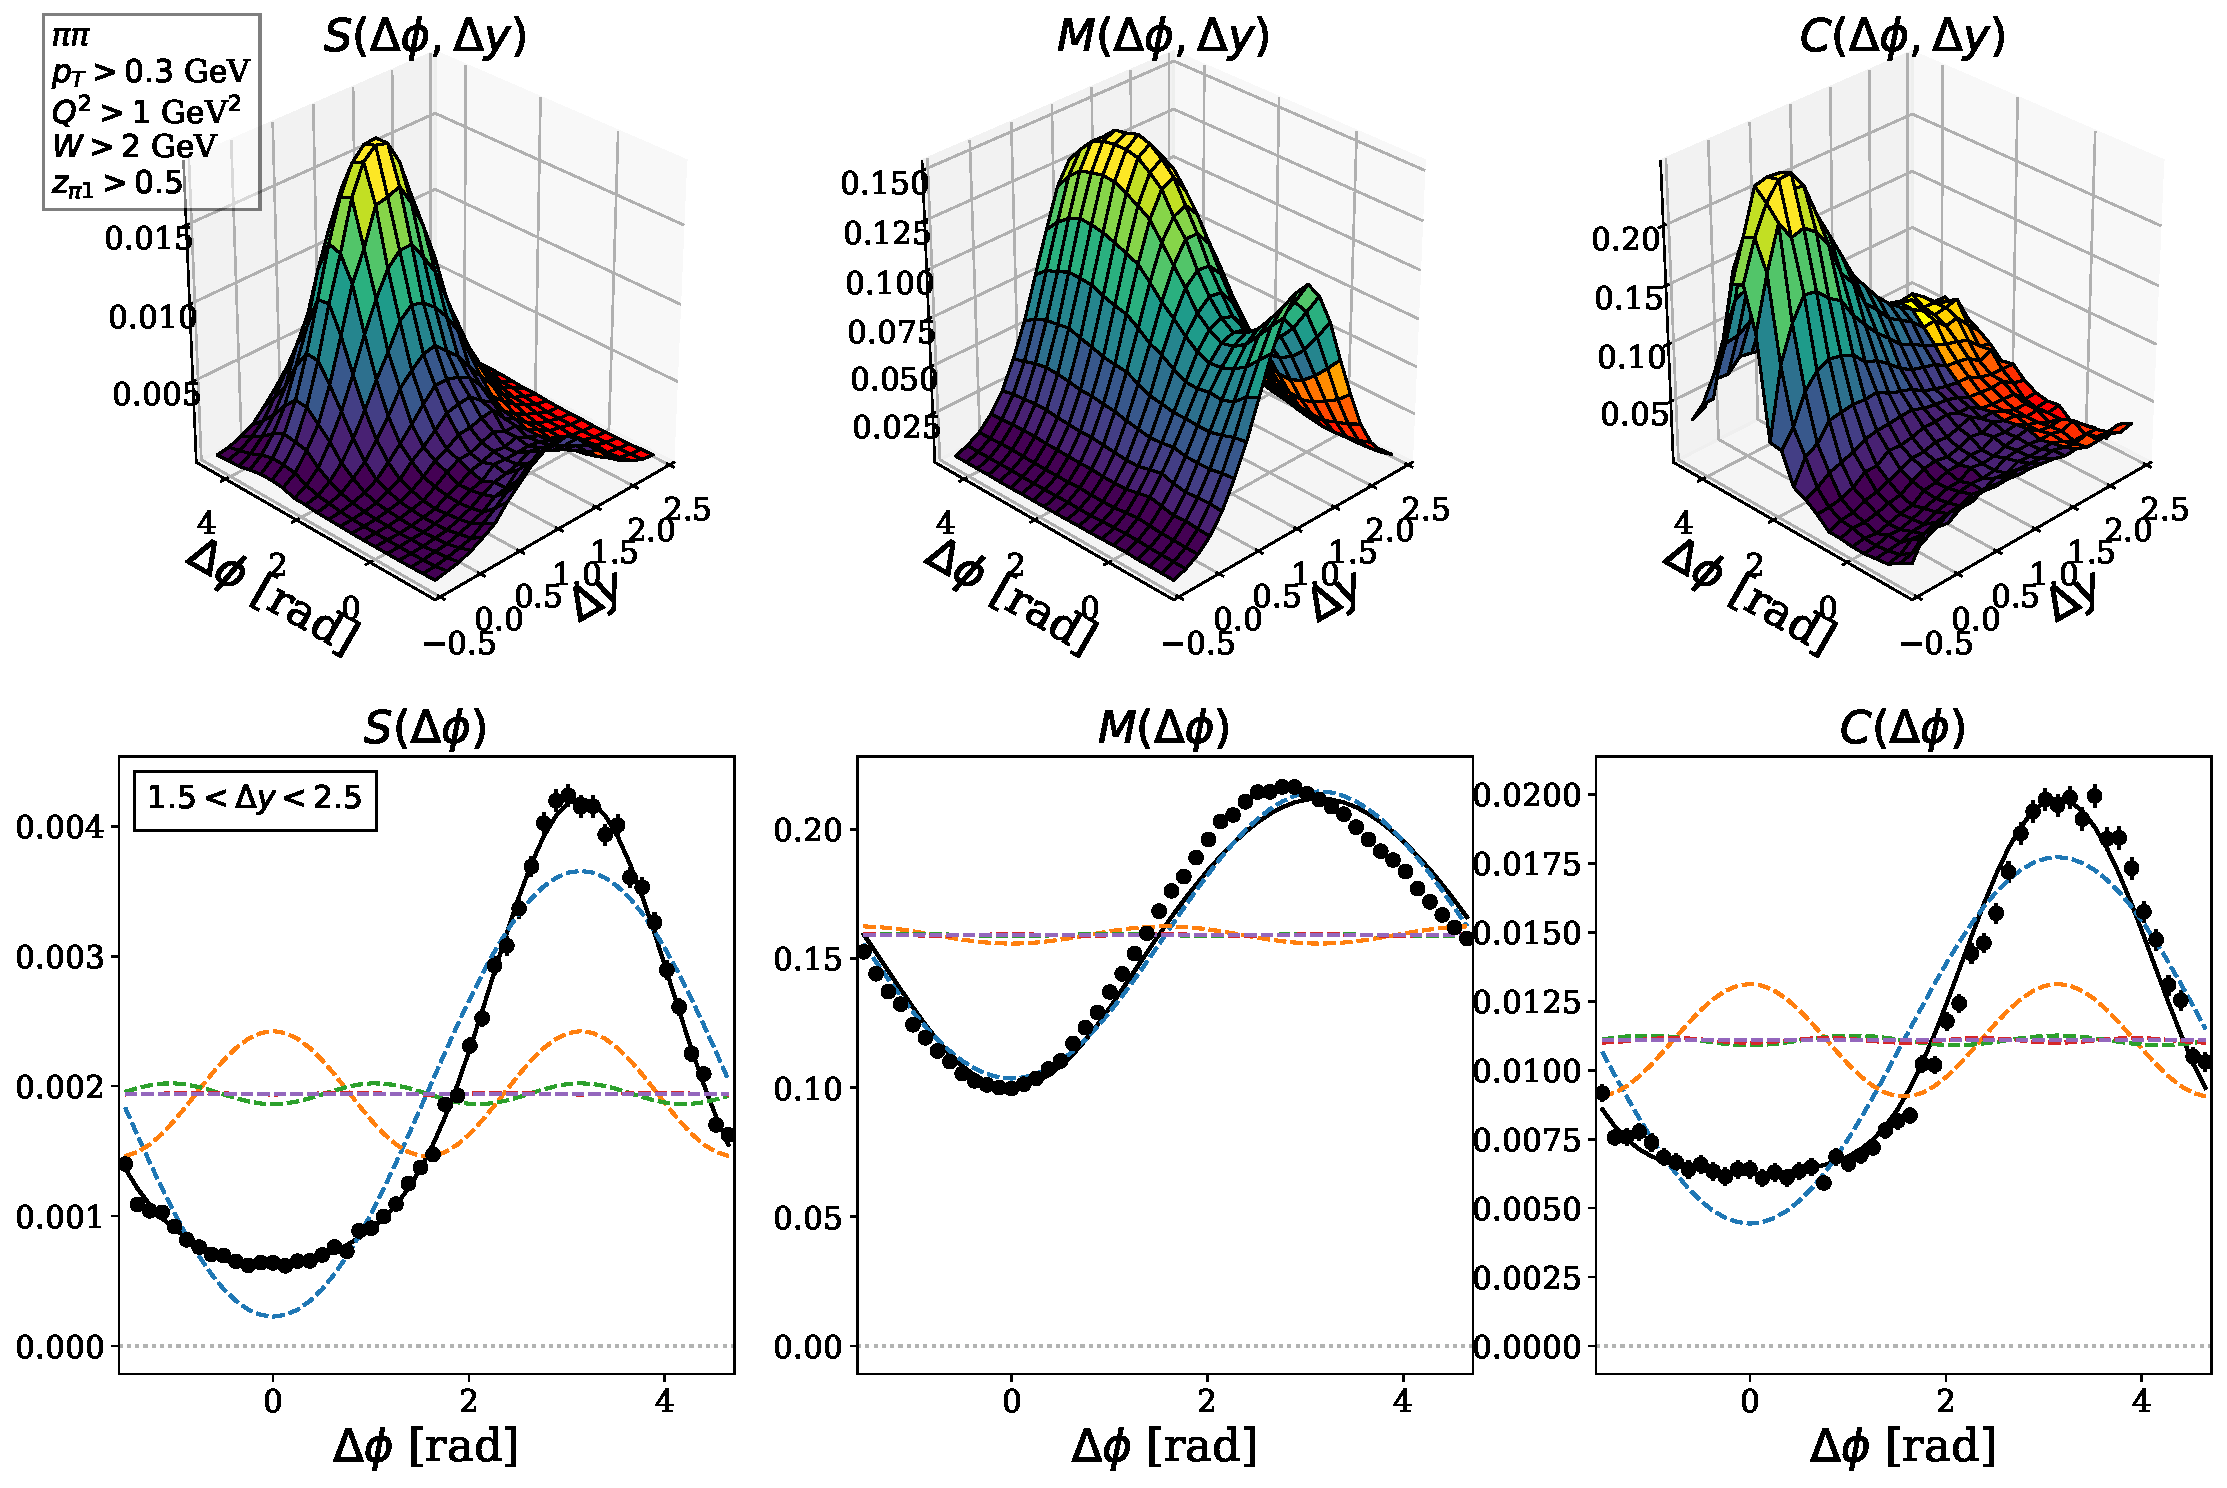
\includegraphics[width=\textwidth]{smc_pi_pi.pdf}
    \caption{Same as Fig.~\ref{fig:corr_pi_p} for $\pi\pi$ events.}
    \label{fig:corr_pi_pi}
\end{figure}

The values of $v_2$ are shown as functions of several kinematic variables in Fig.~\ref{fig:v2_vs_stuff}.  This quantity increases with larger $p_t$ of both hadrons, but it has very little dependance on the $Q^2$.  

\begin{figure}
    \centering
    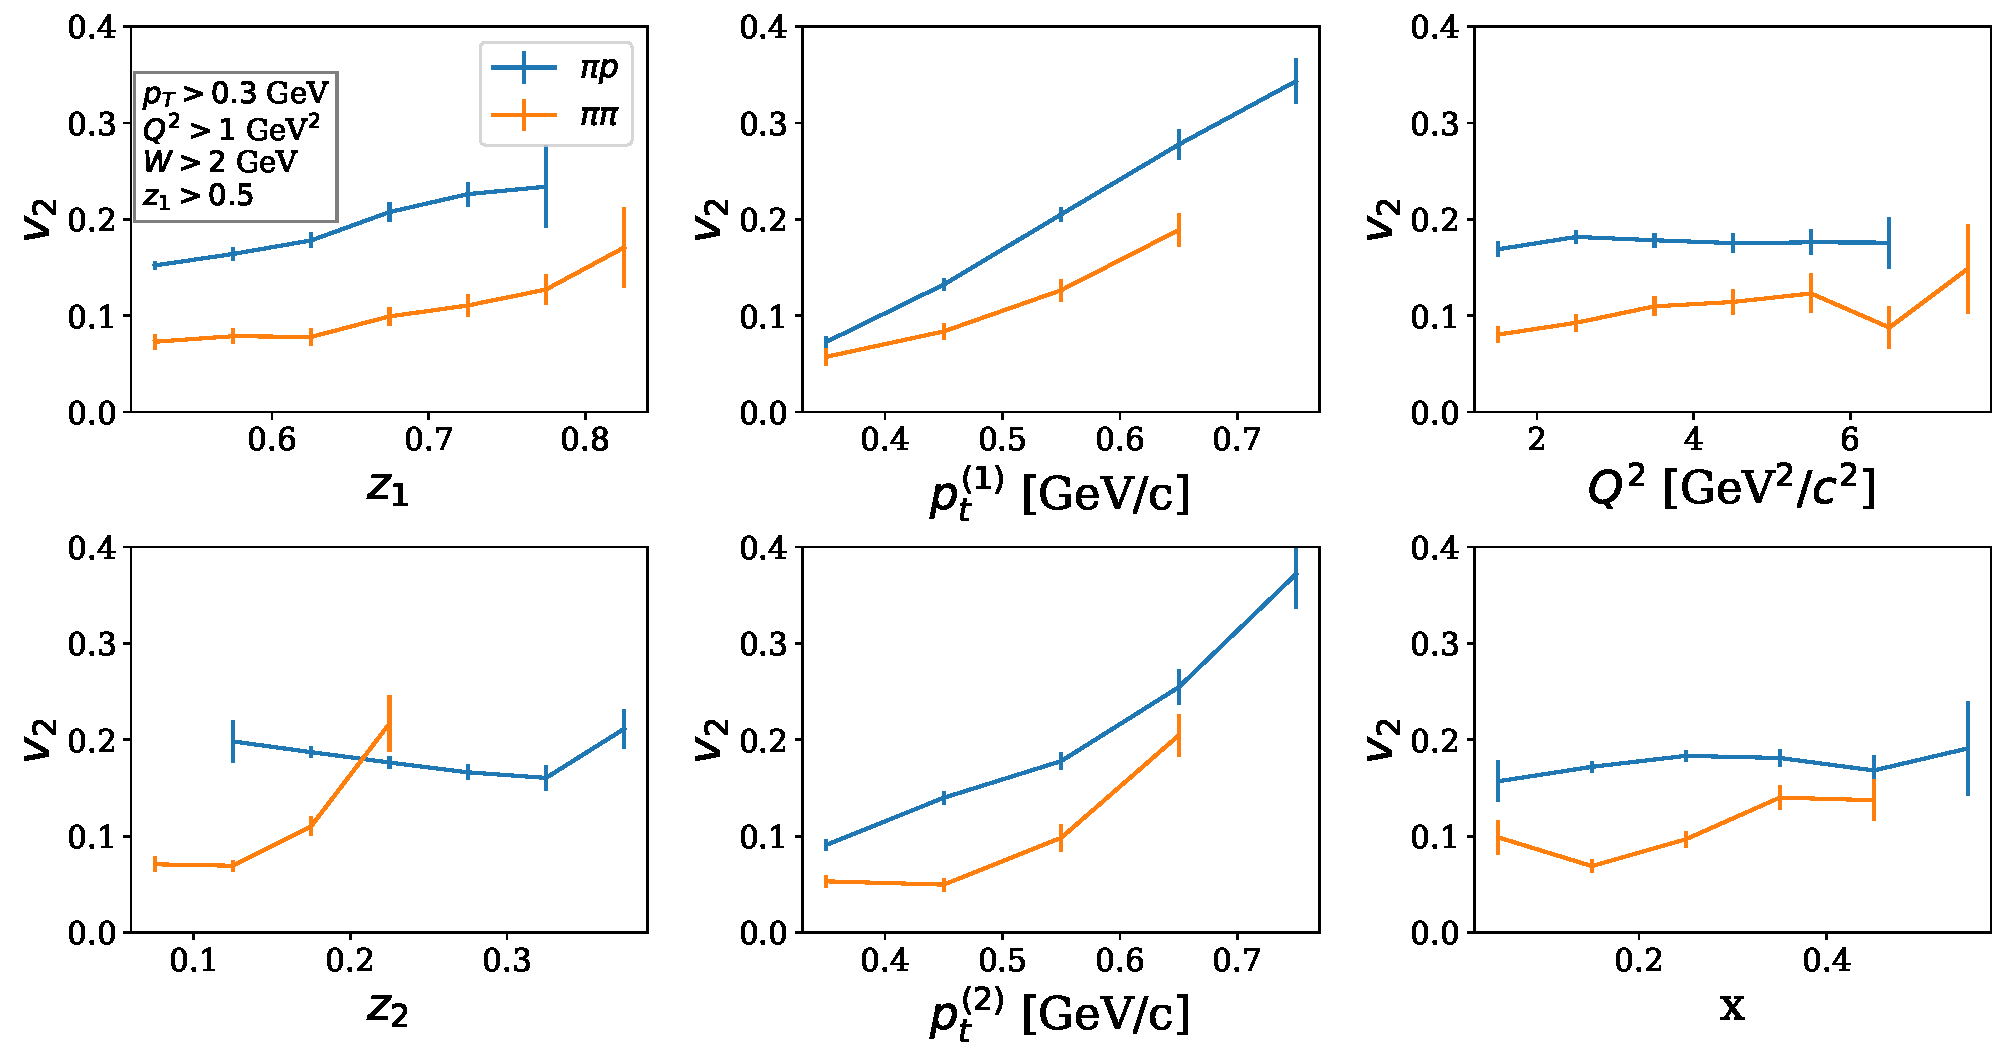
\includegraphics[width=\textwidth]{v2_vs_stuff1.pdf}
    \caption{$v_2$ vs several kinematic variables: $z_1$, $z_2$, etc.}
    \label{fig:v2_vs_stuff}
\end{figure}

The upper limits in the ridge-yield analysis are shown in Fig.~\ref{fig:money_plot} as functions of the track multiplicity, and are compared to results from CMS \cite{Khachatryan:2010gv,CMS:2012qk,Khachatryan:2015lva}, HERA and ALEPH \cite{Lee:2019tmr}.  The correlation functions within each bin in track multiplicity are shown in Fig.~\ref{fig:corrs_vs_ntracks}.  In these plots, we define the track multiplicity to include only \textit{hadronic} tracks passing the cuts in Sec.~\ref{sec:hadron_selection}.  

\begin{figure}
    \centering
    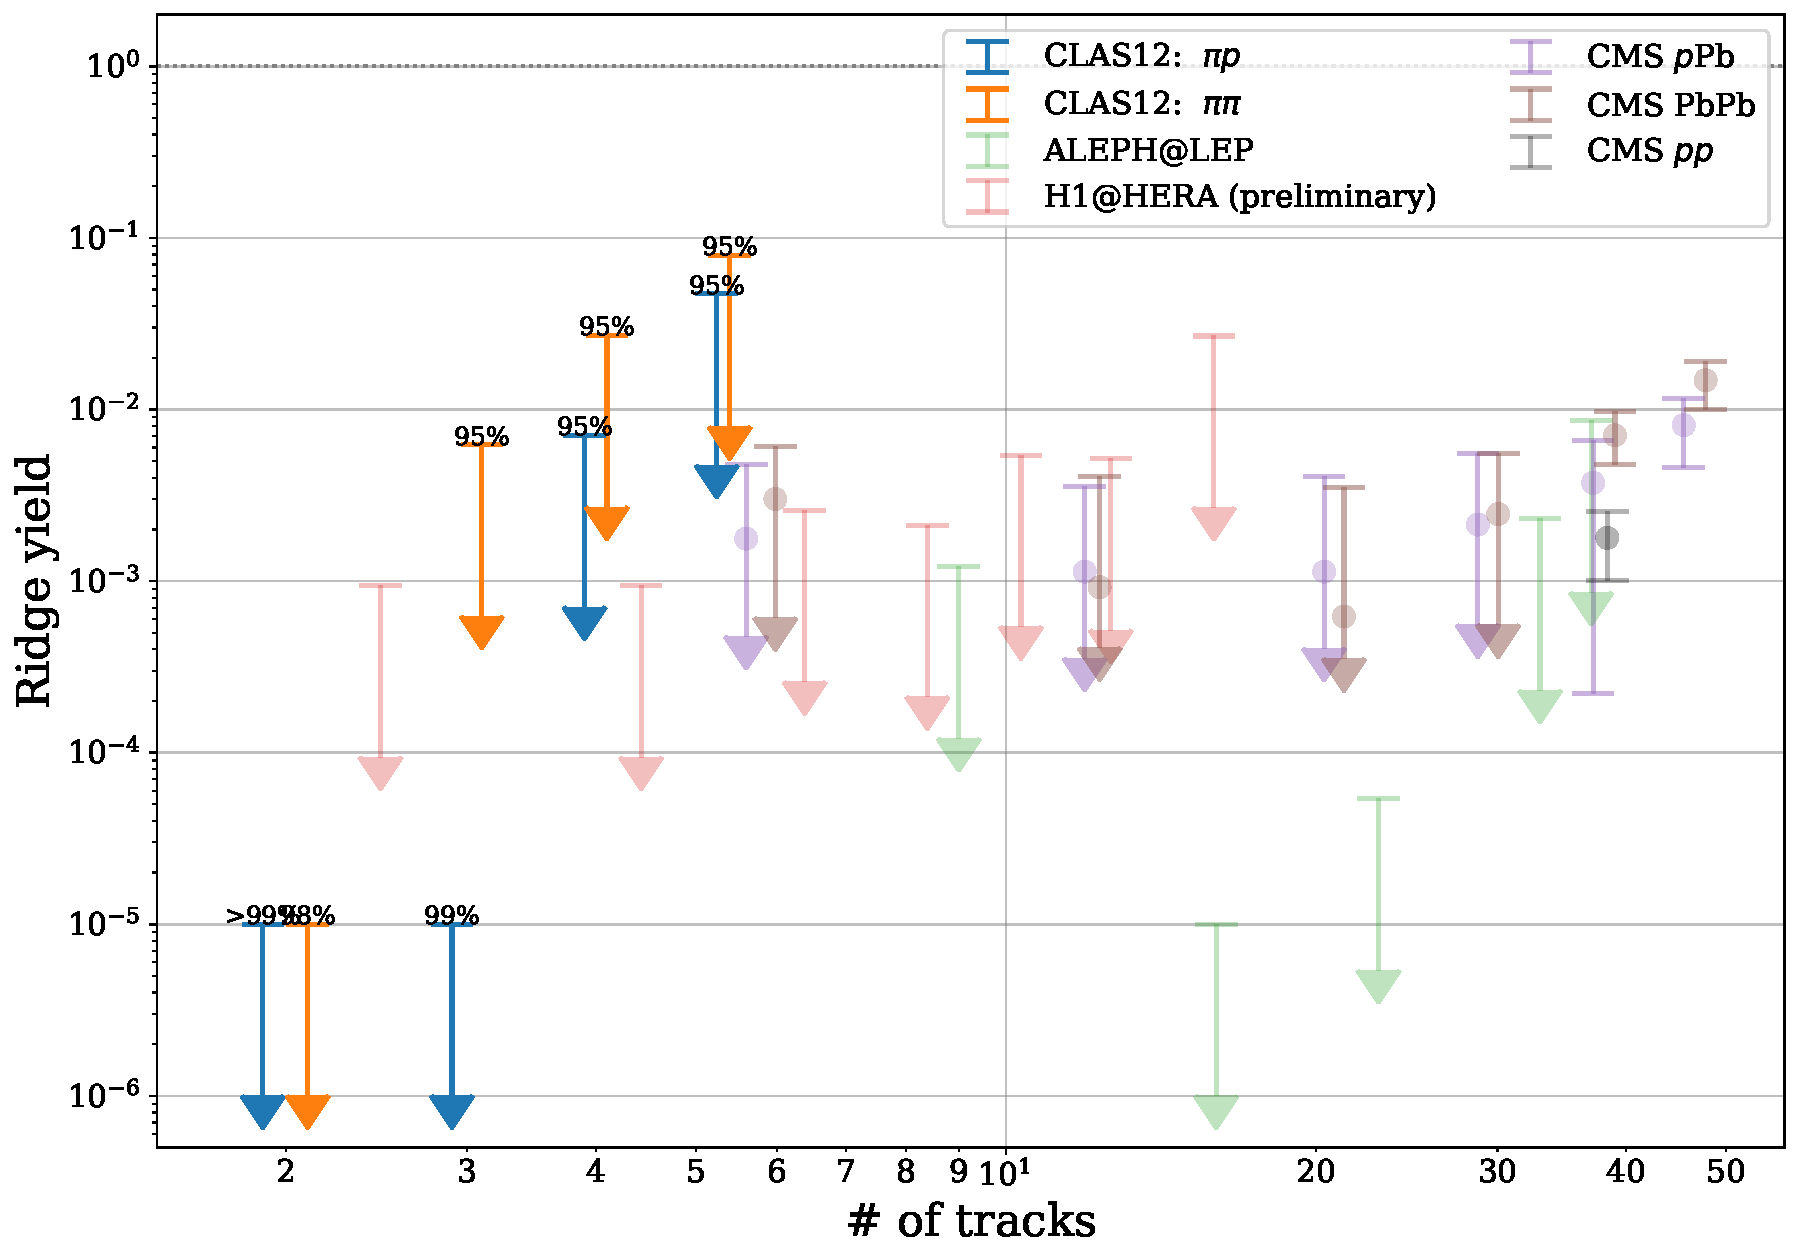
\includegraphics[width=\textwidth]{moneyplot.pdf}
    \caption{Upper limits from ridge-yield analysis in CLAS12, as functions of the track multiplicity.  Superimposed are the results from CMS \cite{Khachatryan:2010gv,CMS:2012qk,Khachatryan:2015lva}, HERA, and ALEPH \cite{Lee:2019tmr}}
    \label{fig:money_plot}
\end{figure}

\begin{figure}
    \centering
    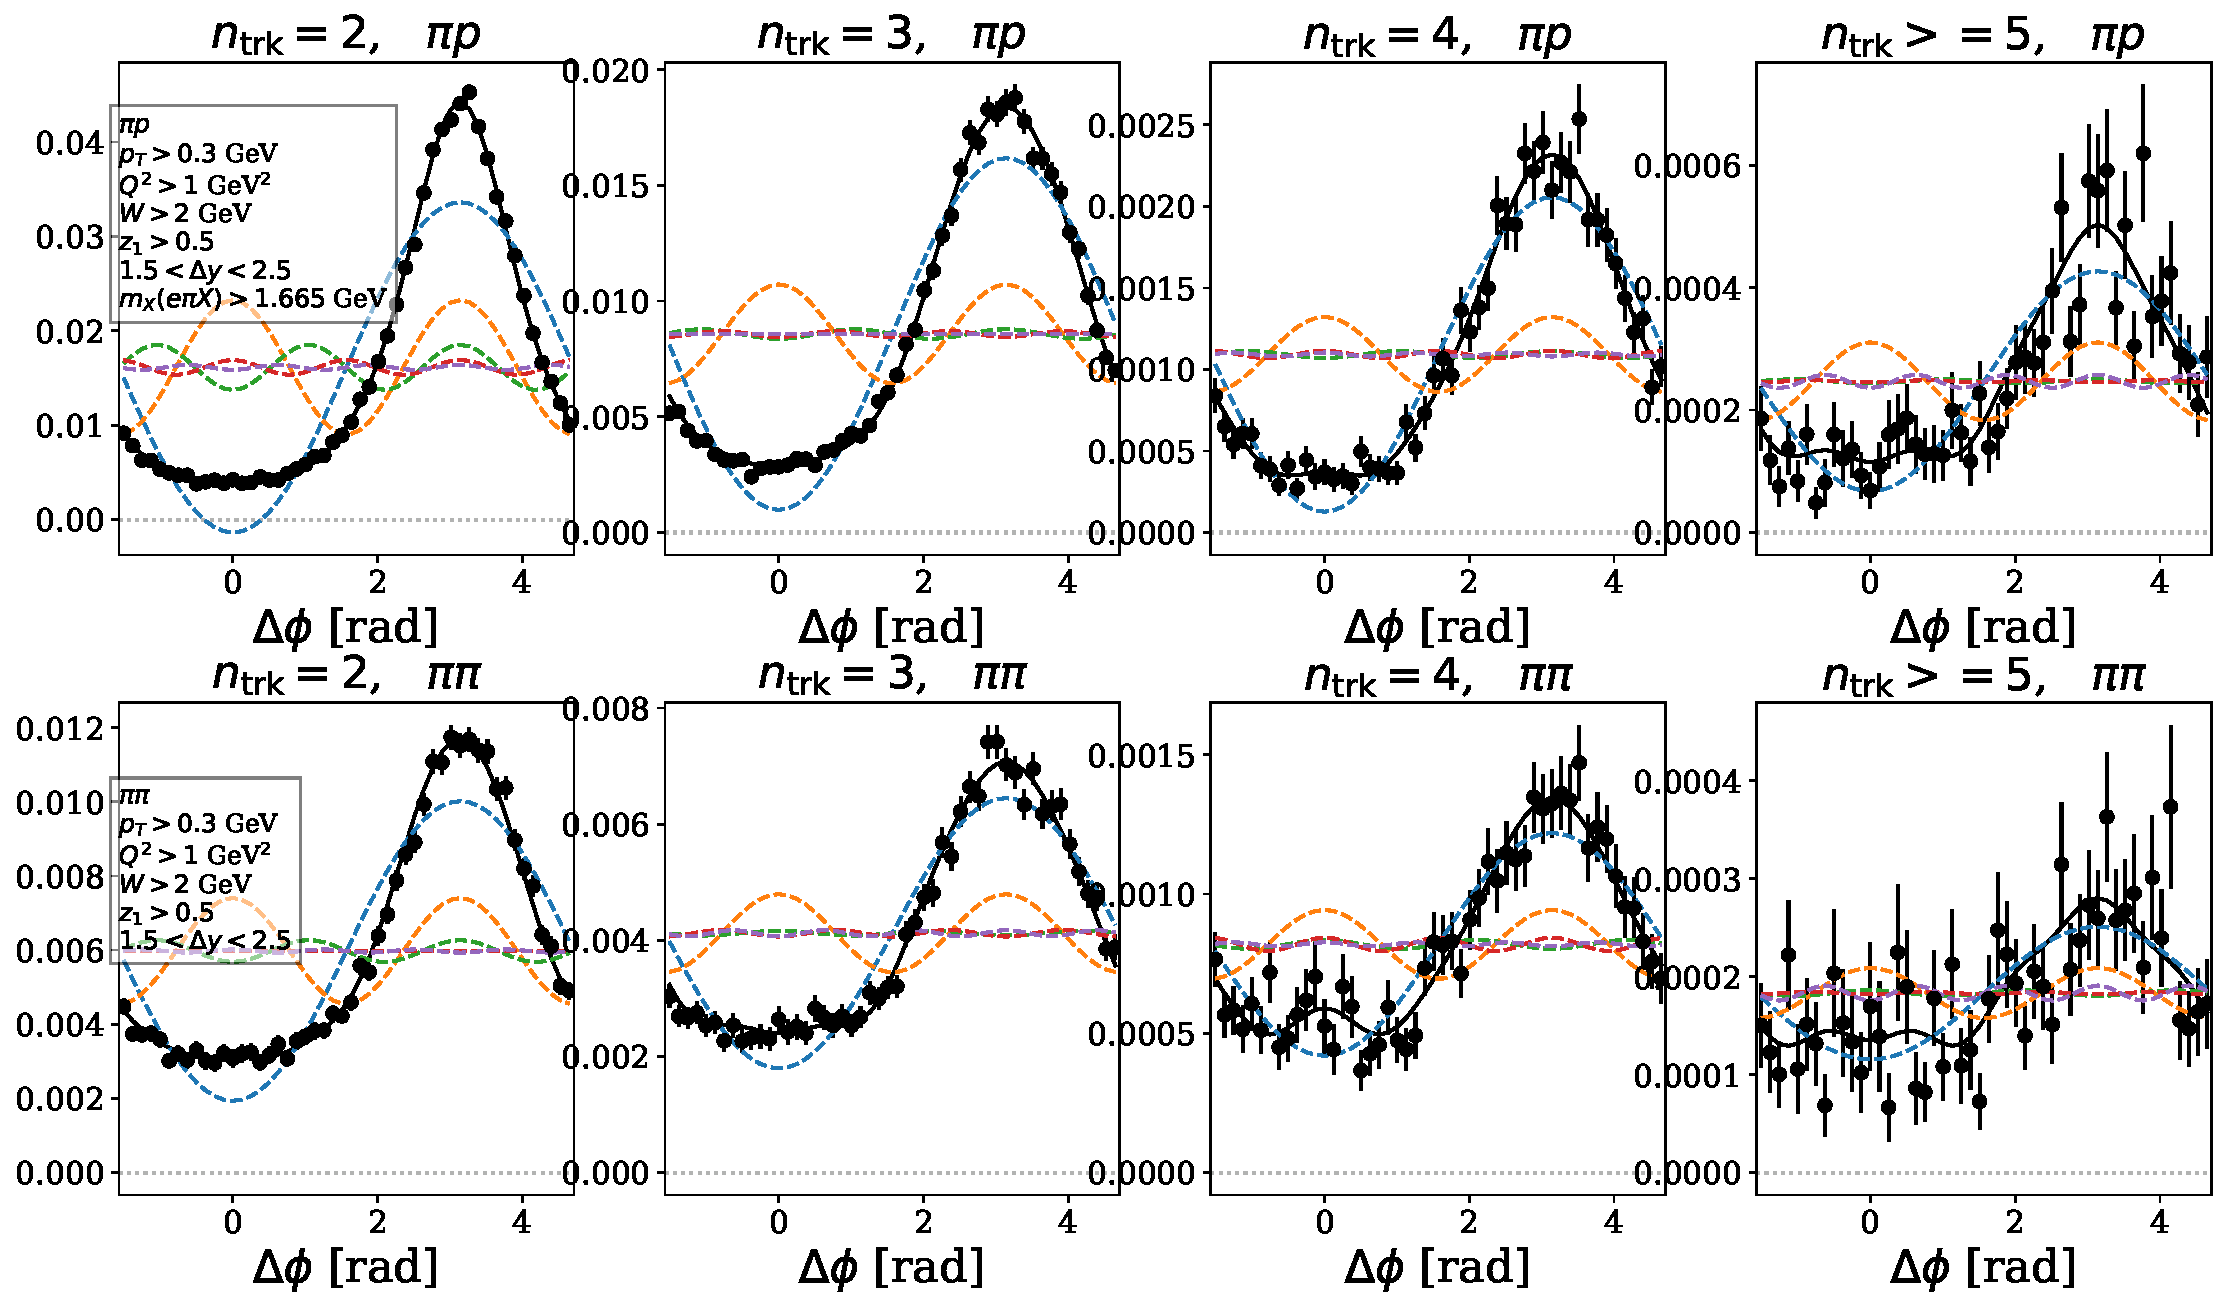
\includegraphics[width=\textwidth]{corrs_vs_ntracks.pdf}
    \caption{Correlation functions for different track-multiplicity bins, for $\pi p$ (top) and $\pi\pi$ events.  These are the same bins used in Fig~\ref{fig:money_plot}.}
    \label{fig:corrs_vs_ntracks}
\end{figure}